\section{What is the LSDF-Portal}

\begin{frame}[standout]
    \Large
    Live Demo!
\end{frame}


\subsection{Overview}

\begin{frame}[c]
    Storage management for 18PB for research projects \\
    Based on Python/django (more on that later) \\
    available at: lsdf.kit.edu \\
    (my test server: lsdf.fkarg.de with user:test and admin4:lsdf) \\
\end{frame}

\subsection{Project Lifecycle}
\begin{frame}[c]
    \begin{itemize}[<+(1)->]
        \item Project Creation -> NEW
        \item Admins take a look -> PENDING
        \item granted -> APPROVED
        \item not granted -> REJECTED
        \item done -> EXPIRED/DELETED
    \end{itemize}
\end{frame}

\subsection{Project Creation}

\begin{frame}[c]{First Login}
                           % trim=left bottom right top, clip
    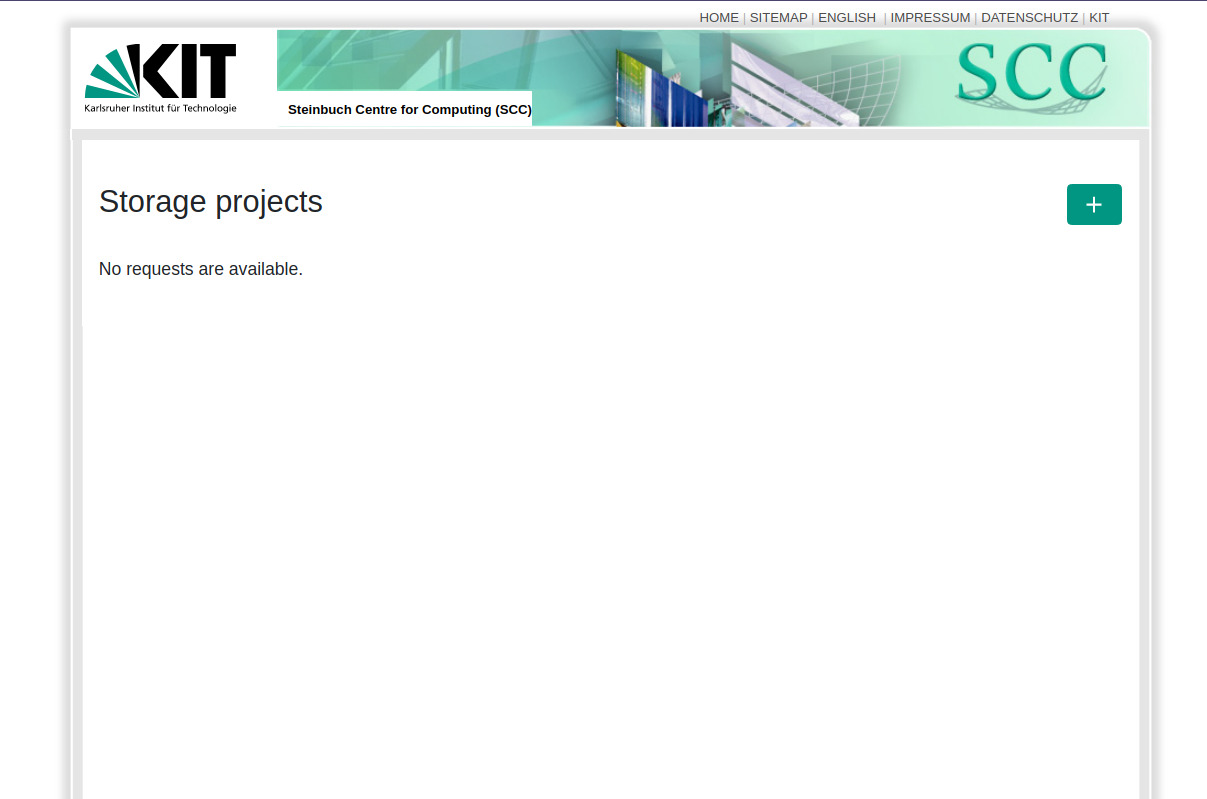
\includegraphics[width=\textwidth,trim=0 0 0 3,clip]{Selection_006}
\end{frame}

\begin{frame}[c]{Project Creation}
                           % trim=left bottom right top, clip
    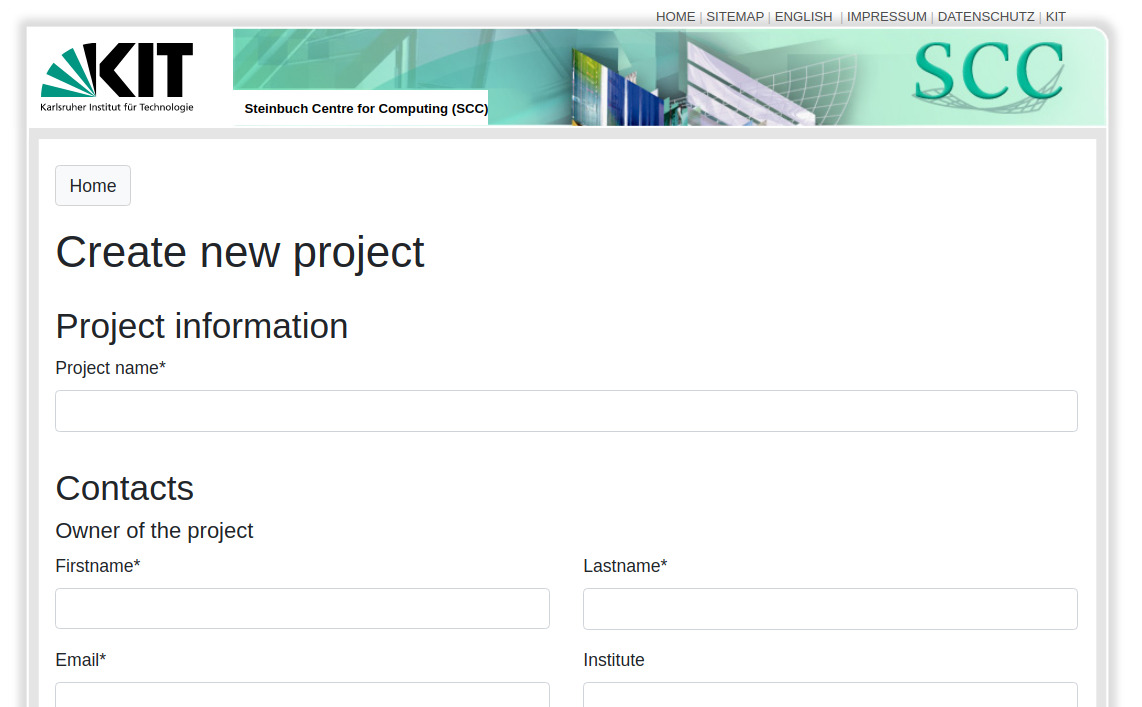
\includegraphics[width=\textwidth,trim=0 0 0 3,clip]{Selection_007}
\end{frame}

\begin{frame}[c]{Project Creation: Add Contacts}
                           % trim=left bottom right top, clip
    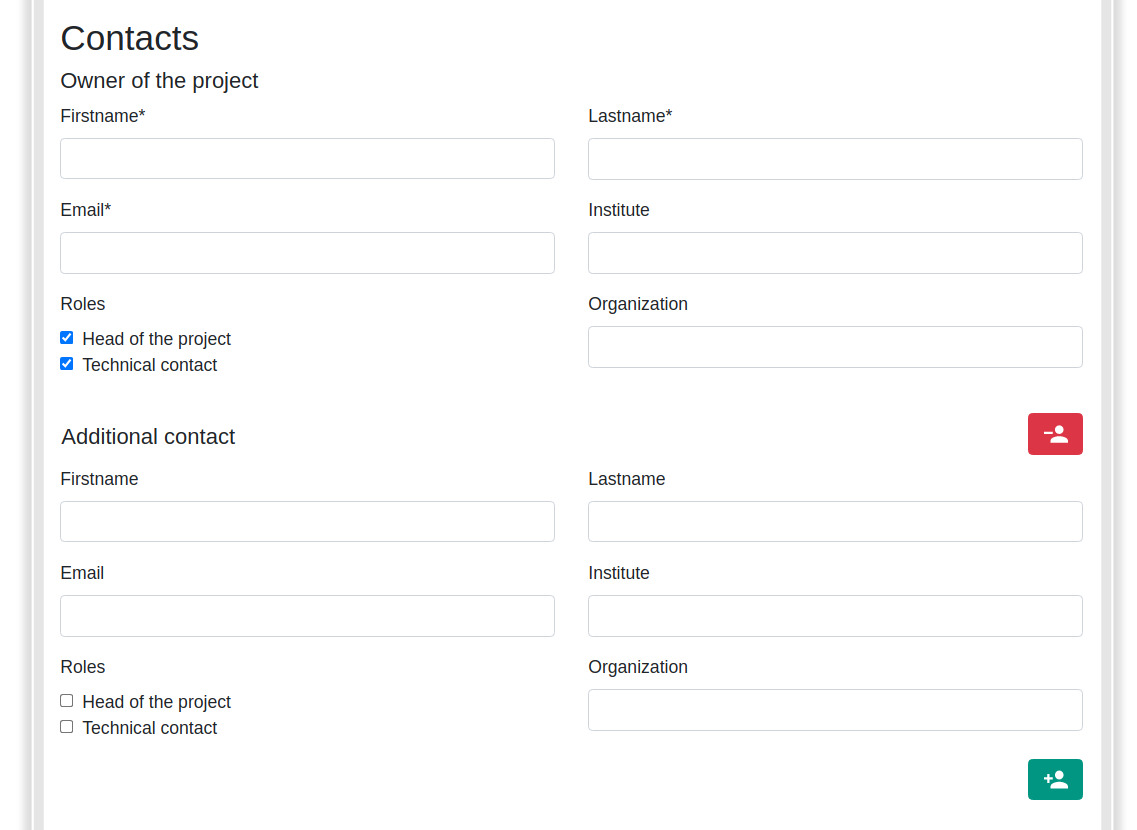
\includegraphics[width=\textwidth,trim=0 0 0 3,clip]{Selection_008}
\end{frame}

\begin{frame}[c]{Available Fields}
                           % trim=left bottom right top, clip
    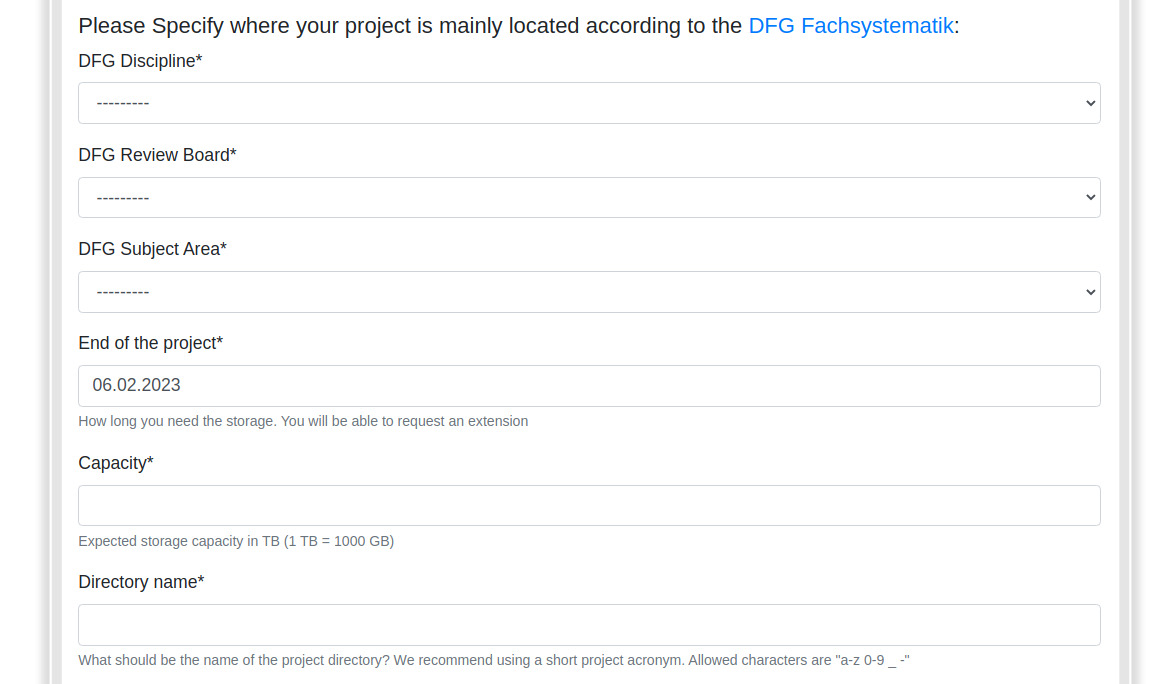
\includegraphics[width=\textwidth,trim=0 0 0 3,clip]{Selection_010}
\end{frame}

\begin{frame}[c]{Fields filled out}
                           % trim=left bottom right top, clip
    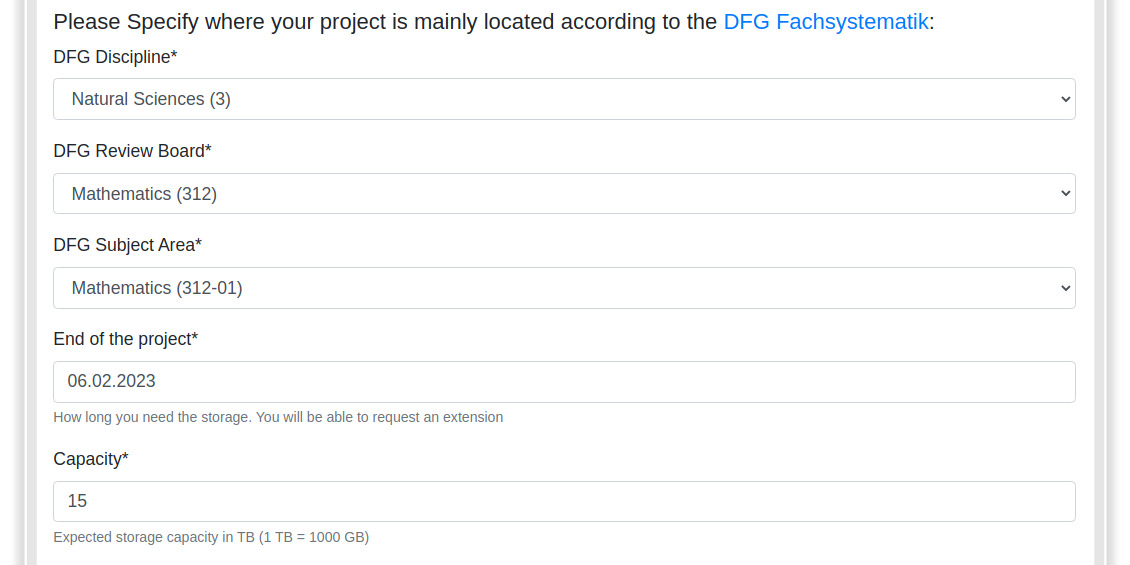
\includegraphics[width=\textwidth,trim=0 0 0 3,clip]{Selection_011}
\end{frame}

\begin{frame}[c]{Submit Proposal}
                           % trim=left bottom right top, clip
    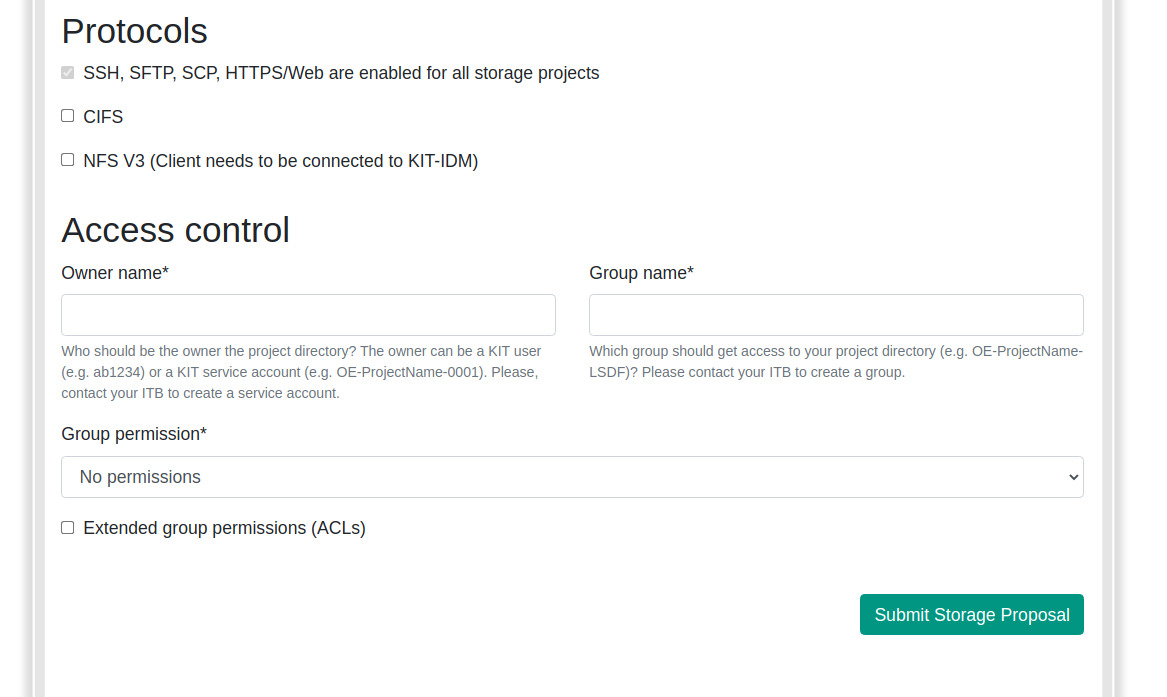
\includegraphics[width=\textwidth,trim=0 0 0 3,clip]{Selection_009}
\end{frame}

\begin{frame}[c]{Succesful Submission}
                           % trim=left bottom right top, clip
    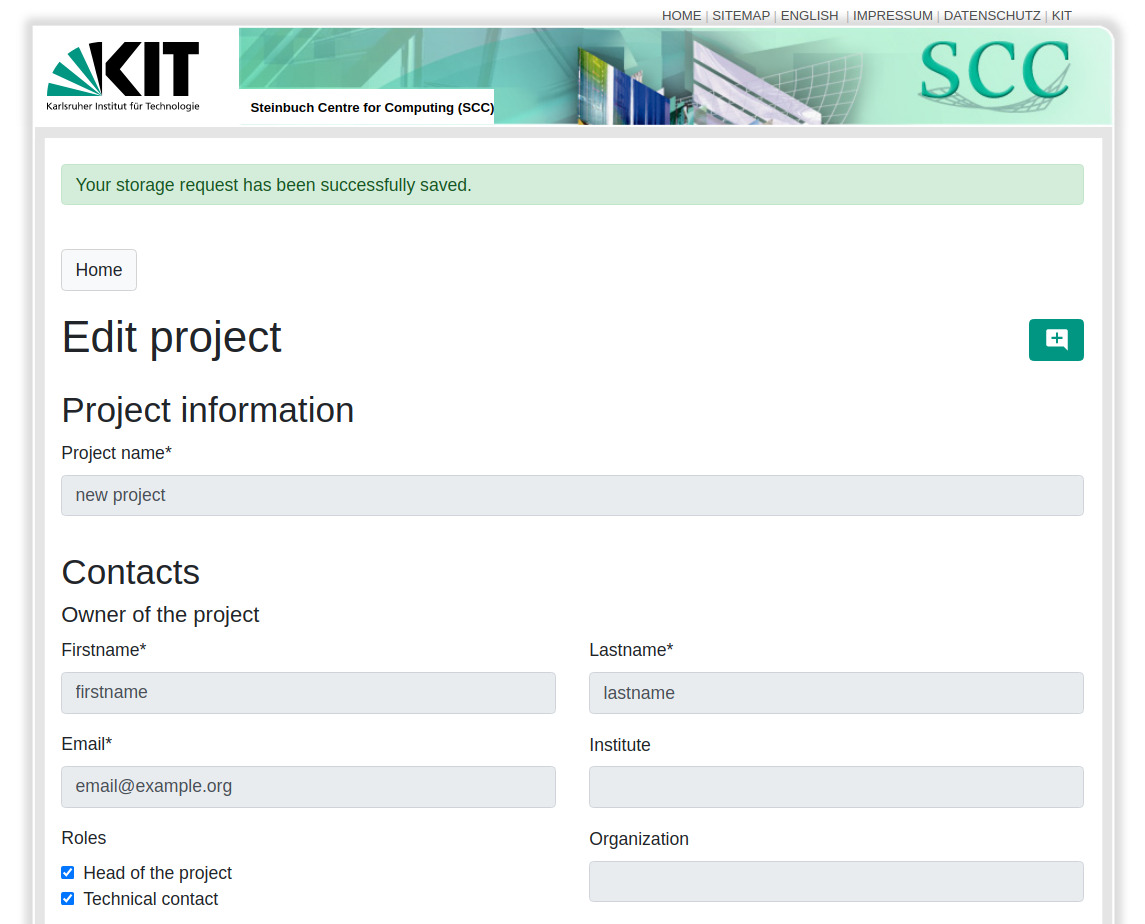
\includegraphics[width=\textwidth,trim=0 0 0 3,clip]{Selection_012}
\end{frame}

\begin{frame}[c]{Project in List}
                           % trim=left bottom right top, clip
    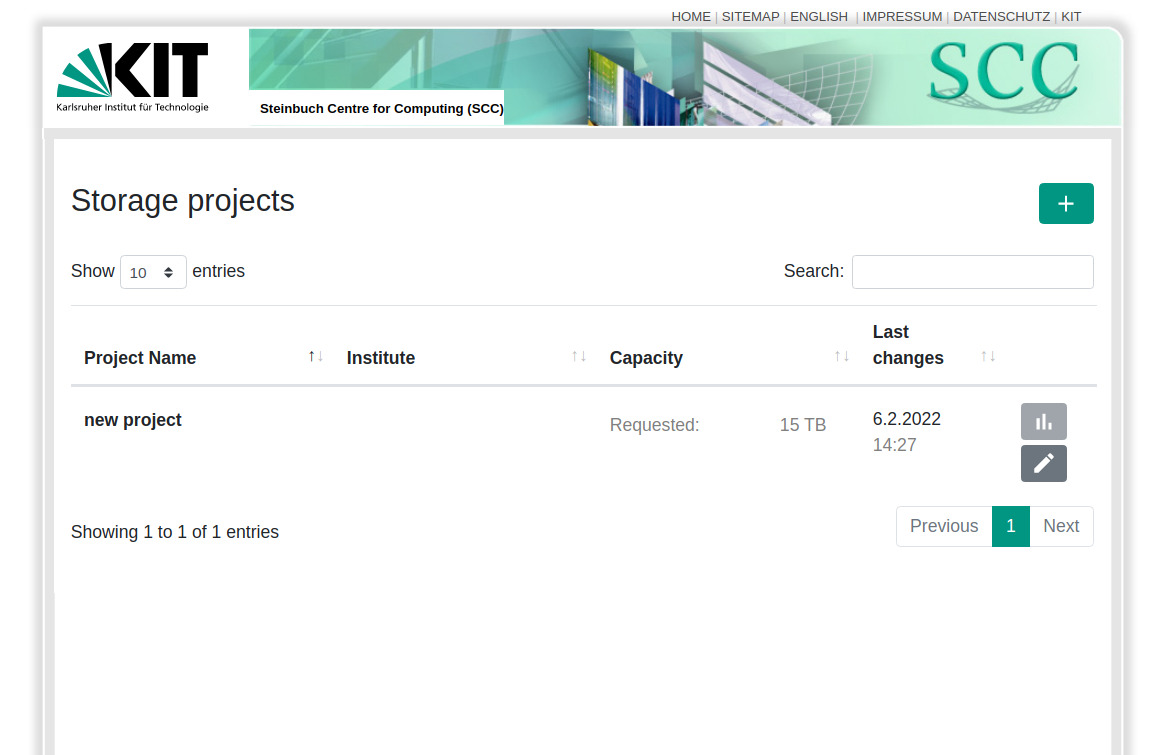
\includegraphics[width=\textwidth,trim=0 0 0 3,clip]{Selection_013}
\end{frame}

\subsection{Project Approval}
\pic{Project Pending}{14}
\pic{State Change Message}{15}
\pic{Project Approved}{17}
\pic{State Change Message}{16}

\subsection{Requesting More Storage}
\pic{Extension Requests: The Project Needs to be Approved}{18}
% \pic{Timeframe Extension Request View}{19}
\pic{lsdf.kit.edu/extension/timeframe/9/create/}{19}
\pic{Capacity Extension Request View}{20}
\pic{Filled out Capacity Extension}{21}
\pic{Extension System Message}{22}

\begin{frame}[c]{Projects Admin View}
                           % trim=left bottom right top, clip
    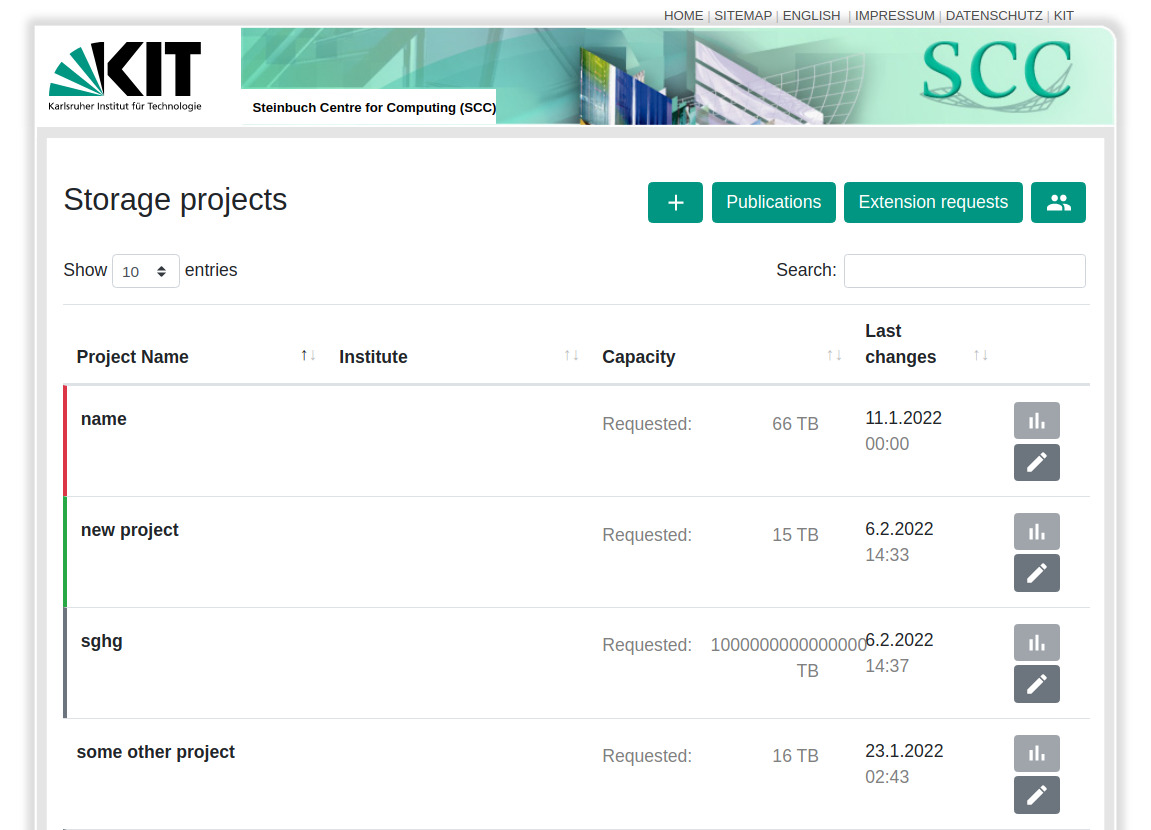
\includegraphics[width=\textwidth,trim=0 0 0 150,clip]{Selection_023}
\end{frame}

% 24 and 25 don't exist
\pic{Extension Request Overview}{26}
\pic{Approving Request}{27}
\pic{System Message showing Extension Approval}{28}
\pic{Increased Capacity from User View}{29}

\begin{frame}[c]{Storage Use Histogram}
    \todo{Screenshot: Histogram of storage usage. } \\
\end{frame}
